\documentclass[12pt]{article}%
\usepackage{amsfonts}
\usepackage{amsmath}
\usepackage{amssymb}
\usepackage{graphicx,tikz}%
\setcounter{MaxMatrixCols}{30}%
\usepackage{graphicx}
%BeginMSIPreambleData
\providecommand{\U}[1]{\protect\rule{.1in}{.1in}}
%EndMSIPreambleData
\newtheorem{theorem}{Theorem}
\newtheorem{acknowledgement}[theorem]{Acknowledgement}
\newtheorem{algorithm}[theorem]{Algorithm}
\newtheorem{axiom}[theorem]{Axiom}
\newtheorem{case}[theorem]{Case}
\newtheorem{claim}[theorem]{Claim}
\newtheorem{conclusion}[theorem]{Conclusion}
\newtheorem{condition}[theorem]{Condition}
\newtheorem{conjecture}[theorem]{Conjecture}
\newtheorem{corollary}[theorem]{Corollary}
\newtheorem{criterion}[theorem]{Criterion}
\newtheorem{definition}[theorem]{Definition}
\newtheorem{example}[theorem]{Example}
\newtheorem{exercise}[theorem]{Exercise}
\newtheorem{lemma}[theorem]{Lemma}
\newtheorem{notation}[theorem]{Notation}
\newtheorem{problem}[theorem]{Problem}
\newtheorem{proposition}[theorem]{Proposition}
\newtheorem{remark}[theorem]{Remark}
\newtheorem{solution}[theorem]{Solution}
\newtheorem{summary}[theorem]{Summary}
\newenvironment{proof}[1][Proof]{\noindent\textbf{#1.} }{\ \rule{0.5em}{0.5em}}
\begin{document}

%\title{Stability in $n$ of graded multiplicities in $S_{n}$ modules}
\title{Stability theorems for multiplicities in graded $S_n$-modules}
\author{Marino Romero \thanks{The author was partially supported by the University of
California President's Postdoctoral Fellowship. }
\and Nolan Wallach}
\maketitle

\begin{abstract}
In this paper, we prove several stability theorems for multiplicities of naturally
defined representations of symmetric groups. The first such theorem states
that if we consider the diagonal action of the symmetric group
$S_{m+r}$ on $k$ sets of $m+r$ variables, then the dimension of the invariants of
degree $m$ is the same as the dimension of the invariants of degree $m$ for
$S_{m}$ acting on $k$ sets of $m$ variables. The second type of stability
result is for Weyl modules. We prove that the dimension of the $S_{n+r}$
invariants for a Weyl module, ${}_{m+r}F^{\lambda}$ (the Schur-Weyl dual of the
$S_{|\lambda|}$ module $V^{\lambda}$) with $\left\vert \lambda \right\vert  \leq
m$ is of the same dimension as the space of $S_{m}$ invariants for
${}_{m}F^{\lambda}$. Multigraded versions of the first type of result are given, as
are multigraded generalizations to non-trivial modules of symmetric groups.
Two related conjectures are given which if proved would give efficient
calculations of multiplicities in the stable range.

\end{abstract}

\section{Introduction}

Consider the diagonal action of the symmetric group on $n$ letters, $S_{n}$,
on $k$ sets of variables. A classical theorem of Hermann Weyl asserts that the
polynomial invariants in $k$ sets of variables are generated by the
polarizations of the invariants in one set of variables. Thus if we take a
standard set, $f_{1},...,f_{n}$, of generators of the symmetric functions in
$n$ variables and do the repeated polarizations to a set of $k$ variables, one
gets a set of generators for the invariants for the diagonal action of the
symmetric group on $k$ sets of variables. A natural question is what are the
relations among these polynomials (the so-called second fundamental theorem)?
In this paper we show that the first relation is in degree $n+2$, which has
the following surprising (at least to us) implication: Looking upon the
diagonal action of $S_{n}$ on $k$ sets of variables as the action of $S_{n}$
on $\mathbb{C}^{k}\otimes\mathbb{C}^{n}$ given by sending $s$ to $I\otimes s$,
if $m\leq n$ then%
\[
\dim S^{m}(\mathbb{C}^{k}\otimes\mathbb{C}^{m})^{S_{m}}=\dim S^{m}%
(\mathbb{C}^{k}\otimes\mathbb{C}^{n})^{S_{n}}.
\]
Here if $M$ is an $S_{n}$ module, $M^{S_{n}}$ is the space of invariants.

In this paper all of the results are true over arbitrary fields of
characteristic $0.$ We state them over $\mathbb{C}$, but they can equally well
be stated and proved in the same way over $\mathbb{Q}$.

This stability theorem is equivalent to another of a different sort. For this
we need some notation. If $\lambda,\mu\in\mathbb{Z}^{n}$ then we will say that
$\lambda\succ\mu$ if
\[
\lambda_{1}+...+\lambda_{i}\geq\mu_{1}+...+\mu_{i}, \text{ for } i=1,...,n.
\]
For $\mu\in\mathbb{Z}^{n}$ we define the character of $\left(  \mathbb{C}%
^{\times}\right)  ^{n},$ thought of as the subgroup of diagonal matrices in
$GL(n,\mathbb{C})$, by
\[
z\mapsto z^{\mu}=z_{1}^{\mu_{1}}z_{2}^{\mu_{2}}\cdots z_{n}^{\mu_{n}}.
\]
If $\lambda=(\lambda_{1},...,\lambda_{r}) \in\mathbb{Z}^{r}$ with $\lambda
_{1}\geq\lambda_{2}\geq...\geq\lambda_{r}\geq0 $ (that is \ $\lambda$ is
dominant) and $r\leq n$, then the theorem of the highest weight implies that
there is a unique up to equivalence irreducible representation of
$GL(n,\mathbb{C})$, ${}_{n}F^{\lambda}$, such that if $\Lambda=(\lambda
_{1},...,\lambda_{r},0,...,0)$ with $n-r$ added $0$'s and if $\mu\in
\mathbb{Z}^{n}$ is such that there exists $v\in$ ${}_{n}F^{\lambda}$ such that
$v\neq0$ and $zv=z^{\mu}v$ for $z \in(\mathbb{C}^{*})^{n}$, then $\Lambda
\succ\mu$. \ Another characterization using the Weyl character formula is that
the character of ${}_{n}F^{\lambda}$ is $s_{\lambda}(z_{1},...,z_{n})$, the
Schur symmetric function.

The so-called $GL(k,\mathbb{C})-GL(n,\mathbb{C})$ duality implies that as a
representation of $GL(k,\mathbb{C})\times GL(n,\mathbb{C})$ the space
$S^{r}(\mathbb{C}^{k}\otimes\mathbb{C}^{n})$ is equivalent to%
\[
\bigoplus_{\left\vert \lambda\right\vert =r}{}_{k}F^{\lambda}\otimes{}%
_{n}F^{\lambda}%
\]
where the sum is over dominant $\lambda$ with at most $\min(k,n)$ entries and
$\left\vert \lambda\right\vert =\sum\lambda_{i} = r$. Using this formalism,
our second main result is as follows. We look upon $S_{n}$ as the group of
permutation matrices in $GL(n,\mathbb{C})$, and for $m \leq n$ we identify
$GL(m,\mathbb{C})$ with the group of matrices
\[
\left\{  \left[
\begin{array}
[c]{cc}%
g & 0\\
0 & I
\end{array}
\right]  \Big| ~g\in GL(m,\mathbb{C})\right\}  .
\]


Then for $\left\vert \lambda\right\vert \leq m\leq n$, the following stability
holds:
\[
\dim\left(  {}_{m}F^{\lambda}\right)  ^{S_{m}}=\dim\left(  {}_{n}F^{\lambda
}\right)  ^{S_{n}}.
\]


In the standard Young correspondence between irreducible representations of
$S_{n}$ and partitions of $n$ in the guise of Young diagrams, the trivial
representation of $S_{n}$ corresponds to the partition $(n)$. If $\mu$ is a
partition of $n$ let $V^{\mu}$ denote the corresponding Young representation
of $S_{n}$. Then if $\mu=(m)$ our result says that
\[
\dim\mathrm{Hom}_{S_{m}}(V^{\mu},{}_{m}F^{\lambda})=\dim\mathrm{Hom}_{S_{m+r}%
}(V^{\mu+re_{1}},{}_{n+r}F^{\lambda})
\]
with $e_{1},...,e_{l}$ the usual basis of $\mathbb{Z}^{l}$. We show that this
stability can be extended to non-trivial representations of the symmetric
group as follows: If $\mu=(\mu_{1},\mu_{2},...)$ is a partition of $m$ and if
$\lambda$ is dominant with
\[
\left\vert \lambda\right\vert \leq m-\mu_{2},
\]
then
\[
\dim\mathrm{Hom}_{S_{m}}(V^{\mu},{}_{m}F^{\lambda})=\dim\mathrm{Hom}_{S_{m+r}%
}(V^{\mu+re_{1}},{}_{m+r}F^{\lambda}).
\]
(Here if $\mu=(\mu_{1})$ then we take $\mu_{2}=0$.) One key aspect of the
proof of this stabilization result is the following result of the first named
author of this paper (see \cite{Rom}). The total degree version found in
Proposition 5.2 of \cite{OZHowe} can also be used to provide an alternate
proof. Considering $S(\mathbb{C}^{k}\otimes\mathbb{C}^{n})$ \ as a
$k$--graded representation of $GL(n,\mathbb{C)}$, $S(\mathbb{C}^{k}%
\otimes\mathbb{C}^{n})$ has a multigrade as follows. If we have $(\mathbb{C}%
^{\times})^{k}$ act on $\mathbb{C}^{k}\otimes\mathbb{C}^{n}$ by $z\mapsto
z\otimes I$ then the $L=(l_{1},...,l_{k})$--level of the grade is the space of
all $v\in S(\mathbb{C}^{k}\otimes\mathbb{C}^{n})$ such that $zv=z_{1}^{l_{1}%
}\cdots z_{k}^{l_{k}}v$ for all $z\in(\mathbb{C}^{\times})^{k}.$ Denote the
$L$--level of the grade by $S^{L}(\mathbb{C}^{k}\otimes\mathbb{C}^{n})$.
Clearly, $S^{L}(\mathbb{C}^{k}\otimes\mathbb{C}^{n})$ is invariant under the
action of $GL(n,\mathbb{C})$ and thus of $S_{n}$. Therefore for any partition
$\mu$,
\[
\mathrm{Hom}_{S_{n}}(V^{\mu},S(\mathbb{C}^{k}\otimes\mathbb{C}^{n}%
))=\bigoplus_{L}\mathrm{Hom}_{S_{n}}(V^{\mu},S^{L}(\mathbb{C}^{k}%
\otimes\mathbb{C}^{n}))
\]
is a grading and there is an associated Hilbert series%
\[
h_{k,n}^{\mu}(q_{1},...,q_{k})=\sum_{L}q_{1}^{l_{1}}q_{2}^{l_{2}}\cdots
q_{k}^{l_{k}}\dim\mathrm{Hom}_{S_{n}}(V^{\mu},S^{L}(\mathbb{C}^{k}%
\otimes\mathbb{C}^{n})).
\]
Fix a monomial order on the monomials in the $q_{1},...,q_{k}$ \ (e.g.
lexicographic order). A semi-standard filling of the Young diagram of $\mu$ is
a placement of monomials in the diagram such that they are in strictly
increasing order in the columns and weakly increasing order in the rows. The
weight of the filling is the product of the monomials in the filling. The
result used is that the coefficient of $q^{L}=q_{1}^{l_{1}}q_{2}^{l_{2}}\cdots
q_{k}^{l_{k}}$ in $h_{k,n}^{\mu}(q_{1},...,q_{k})$ is the number of fillings
if $\mu$ of weight $q^{L}$. This in plethystic notation says
\[
h_{k,n}^{\mu}(q_{1},...,q_{k})=s_{\mu}\left[  \frac{1}{(1-q_{1})\cdots
(1-q_{k})}\right]  .
\]
Contrast this with the corresponding Hilbert series
\[
\sum_{L}q^{L}\dim\mathrm{Hom}_{GL(n,\mathbb{C)}}({}_{n}F^{\lambda}%
,S^{L}(\mathbb{C}^{k}\otimes\mathbb{C}^{n}))=s_{\lambda}(q_{1},...,q_{k}).
\]
So one has%
\[
s_{\mu}\left[  \frac{1}{(1-q_{1})\cdots(1-q_{k})}\right]  =\sum_{\lambda
}s_{\lambda}(q_{1},...,q_{k})\dim\mathrm{Hom}_{S_{n}}(V^{\mu},{}_{n}%
F^{\lambda}).
\]
\newline

The notion of stability of irreducible representations of $S_{n}$ has appeared
in several contexts. For one, the Kronecker coefficients have a stability
condition of Murnaghan \cite{Mur38}, \cite{Mur55}, \cite{KroneckerStability};
and there is stability through the character functions of Orellana and
Zabrocki \cite{OrellanaZabrocki}. More connected to our work,
Church, Ellenberg, and Farb have shown, in their theory of FI-modules
\cite{FImodules}, that Schur functors satisfy a notion of $S_{n}$-stability
for sufficiently large $n$. Some of their stability assertions are made
precise by our identities. Section 4 contains two conjectures that would imply
a simple expression for the graded character of the $S_{n}$ coinvariants up to
degree $n$ (see also \cite{Bergeron}). This expression would also imply the
stability condition for the space of coinvariants, as indicated in \cite{FImodules}.

\section{$S_{n}$ invariants in $S(\mathbb{C}^{k}\otimes\mathbb{C}^{n})$}

We associate to $S(\mathbb{C}^{k}\otimes\mathbb{C}^{n})$ the polynomial ring
\[
\ \mathcal{R} = \mathbb{C}[ {}_{i}x_{1},\dots, {}_{i}x_{n}: i=1,\dots, k ]
\]
in $k$ sets of variables, viewing ${}_{i} x_{j} $ as the generator $e_{i}
\otimes e_{j} \in\mathbb{C}^{k}\otimes\mathbb{C}^{n}.$ The diagonal action of
$s\in S_{n}$ on $\mathcal{R}$ is given by sending ${}_{i}x_{j}$ to ${}%
_{i}x_{s(j)}$ for all $i$. The polynomials of total degree $d$ will be denoted
by $\mathcal{R}_{d}$, and we let $\mathcal{R}_{\leq d}$ denote the space of
polynomials of total degree at most $d$.

A basis for the $S_{n}$ invariants of $\mathcal{R}$ can be found by first
choosing a monomial
\[
x^{\alpha}= \prod_{i=1}^{k} \prod_{j=1}^{n} {}_{i}x_{j}^{ {}_{i}\alpha_{j}}%
\]
and taking the sum of the orbit $S_{n}(x^{\alpha})$. Note that the orbit
corresponds to taking the sequence of vectors $(P^{1}(\alpha) ,\dots,
P^{n}(\alpha))$, with
\[
P^{i}(\alpha) = ({}_{1}\alpha_{i},\dots, {}_{k}\alpha_{i}),
\]
and permuting the vectors in all possible ways, since $S_{n}$ acts diagonally.
This means that a representative of the orbit is the multiset of sequences
$P^{\alpha}= [P^{1}(\alpha) ,\dots, P^{n}(\alpha)].$ In other words, we look
at the set created by $P^{1}(\alpha) ,\dots, P^{n}(\alpha)$, including multiplicities.

The dimension of invariants of degree equal to $d$ is equal to the cardinality
of the set $\mathcal{P}_{d}^{n,k}$ of multisets $[P^{1},\dots,P^{n}]$ such
that each $P^{i}=(P_{1}^{i},\dots,P_{k}^{i})$ is a sequence of $k$ nonnegative
integers satisfying
\[
|P^{1}|+\cdots+|P^{n}|=d\text{ with }|P^{i}|=P_{1}^{i}+\cdots+P_{k}^{i}.
\]
The union of all $\mathcal{P}_{d}^{n,k}$ with $d\leq r$ will be denoted by
$\mathcal{P}_{\leq r}^{n,k}$. This implies, for the space of polynomials with
degree less than or equal to $d$, that
\[
\dim\mathcal{R}_{\leq d}^{S_{n}}=|\mathcal{P}_{\leq d}^{n,k}|.
\]


In \cite{Weyl}, Weyl showed that a set of generators for the invariants is
given by the polarized power sums
\[
p_{a}=p_{(a_{1},\dots,a_{k})}=\sum_{i=1}^{n}{}_{1}x_{i}^{a_{1}}\cdots{}%
_{k}x_{i}^{a_{k}}%
\]
with $0<|a|=a_{1}+\cdots+a_{k}\leq n$. In other words, every invariant can be
written as a polynomial in the polarized power sums of degree at most $n$.

The number of monomials $p_{a^{1}}\cdots p_{a^{r}}$ we can construct whose
total degree is less than or equal to $n$ is the same as picking a multiset of
sequences
\[
\left[  a^{1}=(a_{1}^{1},\dots,a_{k}^{1}),\dots,a^{r}=(a_{1}^{r},\dots
,a_{k}^{r})\right]  ,
\]
each with a nonzero entry, such that $|a^{1}|+\cdots+|a^{r}|\leq n$. Note
however that since each $a^{i}$ has a nonzero entry, there are at most $n$ of
them. This is in bijection with the set $\mathcal{P}_{\leq n}^{n,k}$ by adding
a sufficient number of sequences whose only entries are zeroes. This proves
that the set
\[
\{p_{a^{1}}\cdots p_{a^{r}}:|a^{1}|+\cdots+|a^{r}|\leq n\}
\]
is not only a spanning set for the space of invariants of degree at most $n$,
but also a basis. Surprisingly, there is a stronger independence satisfied by
these monomials.

\begin{theorem}
The collection
\[
\{p_{a^{1}}\cdots p_{a^{r}}:|a^{1}|+\cdots+|a^{r}|\leq n+1\}
\]
is a basis for $\mathcal{R}_{\leq n+1}^{S_{n}}$.
\end{theorem}

\begin{proof}
We have shown that the set of monomials $p_{a^{1}}\cdots p_{a^{r}}$ of degree
at most $n$ are a basis for the invariants of degree at most $n$. For
monomials of degree $n+1$, we have to show that the number of possible
monomials in the polarized power sums of degree $n+1$ is equal to the
cardinality of $\mathcal{P}_{n+1}^{n,k}$.

An element $[P^{1},\dots, P^{n}] \in\mathcal{P}^{n,k}_{n+1}$ falls into one of
two cases:

\begin{enumerate}
\item $|P^{i}| \leq n$ for all $i$, or

\item there is an $i$ for which $|P^{i}| =n+1$.
\end{enumerate}

In the first case, we have the monomial
\[
p_{P^{1}}\cdots p_{P^{n}}.
\]
The convention here gives $p_{P^{i}} = 1$ for $P^{i} = (0,\dots, 0)$. This
accounts for all monomials in the polarized power sums with at most $n$
factors. In the second case, we may assume that $|P^{1}|=n+1$ and $|P^{i}|=0$
for $i>1$. The number of such choices is the number of ways of choosing
$P^{1}=(a_{1},\dots,a_{k})$ with
\[
a_{1}+\cdots+a_{k}=n+1,
\]
giving the binomial coefficient
\[
\binom{n+1+k-1}{k-1}=\binom{n+k}{k-1}.
\]
On the other hand, a monomial in the polarized power sums $p_{a^{1}}\cdots
p_{a^{n+1}}$ is of degree $n+1$ precisely when $|a^{i}|=1$ for all $i$. Let
$a_{j}$ be the number of $a^{i}$ whose component $j$ is nonzero. Then picking
such a monomial is equivalent to choosing $a_{1}+\cdots+a_{k}=n+1$, meaning
the number of such choices is again $\binom{n+k}{k-1}$. This shows that the
set of monomials in the polarized power sums whose degree is at most $n$ is a
basis for the invariants of degree at most $n+1$.
\end{proof}

We put the standard symmetric bilinear form $\left\langle (z_{1}%
,...,z_{k}),(w_{1}...,w_{k})\right\rangle =\sum z_{i}w_{i}$ on $\mathbb{C}%
^{k}$. On $\mathbb{C}^{k}\otimes\mathbb{C}^{n}$ we use the tensor product of
the forms on $\mathbb{C}^{k}$ and $\mathbb{C}^{n}$. This form is invariant
under the action of $S_{n}$ given by $\sigma(v\otimes w)=v\otimes\sigma w.$
Then $\mathcal{R}_{d}$ is isomorphic with $S^{d}(\mathbb{C}^{k}\otimes
\mathbb{C}^{n})$, using the form to identify $\mathbb{C}^{k}\otimes
\mathbb{C}^{n}$ with $(\mathbb{C}^{k}\otimes\mathbb{C}^{n})^{\ast}$. Thus we have

\begin{corollary}
\label{dimthm}For $r\leq m\leq n$,
\[
\dim S^{r}(\mathbb{C}^{k}\otimes\mathbb{C}^{m})^{S_{m}}=\dim S^{r}%
(\mathbb{C}^{k}\otimes\mathbb{C}^{n})^{S_{n}}%
\]
and
\[
\sum_{n=1}^{\infty}\dim S^{n}(\mathbb{C}^{k}\otimes\mathbb{C}^{n})^{S_{n}%
}q^{n}=%
%TCIMACRO{\dprod _{n=1}^{\infty}}%
%BeginExpansion
{\displaystyle\prod_{n=1}^{\infty}}
%EndExpansion
\frac{1}{(1-q^{r})^{\binom{r+k-1}{k-1}}}%
\]

\end{corollary}

\begin{proof}
In the above notation, we have that $\mathcal{R}_{r}^{S_{n}}=S^{r}%
(\mathbb{C}^{k}\otimes\mathbb{C}^{n})^{S_{n}}$ has dimension equal to
$|\mathcal{P}_{r}^{n,k}|$. It is therefore sufficient to show that
$|\mathcal{P}_{r}^{m,k}|=|\mathcal{P}_{r}^{n,k}|$. Since $n\geq m$, any
element $[P^{1},\dots,P^{n}]\in\mathcal{P}_{r}^{n,k}$ must have at most $r
\leq m$ nonzero $P^{i}$. Therefore, the map that takes $P\in\mathcal{P}%
_{r}^{m,k}$ and adds $n-m$ zero vectors is not only injective, but also
surjective. The two sets then have the same cardinality, and the equality holds.

We will now prove the sum product formula. We have shown that
\[
\dim S^{n}(\mathbb{C}^{k}\otimes\mathbb{C}^{n})^{S_{n}}=|\{p_{a^{1}}\cdots
p_{a^{r}}:|a^{1}|+\cdots+|a^{r}|=n\}|,
\]
which is the coefficient of $q^{n}$ in the generating series
\[
\prod_{a}\frac{1}{1-q^{|a|}},
\]
where the product runs over all nonzero $a\in\mathbb{Z}_{\geq 0}^{k}$. This product is
independent of $n$, and the factor $1/1-q^{r}$ appears with multiplicity the
number of $a$ with $|a|=r$. The number of $a=(a_{1},...,a_{k})$ satisfying
$\sum a_{i}=r$ is given by the binomial coefficient $\binom{r+k-1}{k-1}$.
\end{proof}

Recall that if $k,n\in\mathbb{Z}_{>0}$ then $\otimes^{k}\mathbb{C}^{n}$ is a
module for $S_{k}\times GL(n,\mathbb{C})$ with $s\in S_{k}$ permuting the
tensor factors and $g\in GL(n,\mathbb{C})$ acting by $\otimes^{k}g$. As a
representation of $S_{k}\times GL(n,\mathbb{C})$, the module $\otimes
^{k}\mathbb{C}^{n}$ decomposes according to Schur-Weyl duality (c.f.
\cite{GW},9.1.1) as follows:
\[
\otimes^{k}\mathbb{C}^{n}\cong\bigoplus_{%
\begin{array}
[c]{c}%
\lambda\dashv k\\
\ell(\lambda)\leq\min\{n,k\}
\end{array}
}V^{\lambda}\otimes{}_{n}F^{\lambda}.
\]
Here, $V^{\lambda}$ is the Young module for $S_{k}$ corresponding to the
partition $\lambda=(\lambda_{1}\geq\cdots\geq\lambda_{r}>0)$ of size
$|\lambda|=\lambda_{1}+\cdots+\lambda_{r}=k$ with length $\ell(\lambda)=r$;
and ${}_{n}F^{\lambda}$ is the Weyl module for $GL(n,\mathbb{C})$
corresponding to $\lambda$. Let $\epsilon(\lambda)=\sum_{i=1}^{r}\lambda
_{i}\varepsilon_{i}$. Here, $\varepsilon_{i}$ is the linear functional on the
space of diagonal matrices
\[
h=\left[
\begin{array}
[c]{cccc}%
h_{1} & 0 & \cdots & 0\\
0 & h_{2} & \cdots & 0\\
\vdots & \vdots & \ddots & \vdots\\
0 & 0 & \cdots & h_{n}%
\end{array}
\right]
\]
given by $\varepsilon_{i}(h)=h_{i}$. The space $\mathfrak{h}$ of diagonal
$n\times n$ matrices is a Cartan subalgebra of $M_{n}(\mathbb{C})$, the Lie
algebra of $GL(n,\mathbb{C})$; and ${}_{n}F^{\lambda}$ is the irreducible
representation of $GL(n,\mathbb{C})$ with highest weight $\epsilon(\lambda)$
relative to the choice of positive roots $\varepsilon_{i}-\varepsilon_{j}$,
$1\leq i<j\leq n$. 

Consider the subgroup $GL(n-1,\mathbb{C})$ of $GL(n,\mathbb{C})$ consisting of
the matrices%
\[
\left\{  \left[
\begin{array}
[c]{cc}%
g & 0\\
0 & 1
\end{array}
\right]  \Big| ~g\in GL(n-1,\mathbb{C})\right\}  .
\]
Let $\mu=\sum_{i=1}^{n}\mu_{i}\varepsilon_{i}$ with $\mu_{i}\in\mathbb{Z}%
_{\geq0}$ and $\mu_{i}\geq\mu_{i+1}$ for all $i=1,\dots,n-1$ (that is, $\mu$ is
a dominant integral weight). The branching theorem (c.f. \cite{GW},Theorem
8.1.1) implies that if we consider ${}_{n}F^{\mu}$ to be a $GL(n-1,\mathbb{C}%
){}$ module, then
\[
{}_{n}F^{\mu}\Big|_{ GL(n-1,\mathbb{C})} \cong\bigoplus_{%
\begin{array}
[c]{c}%
\nu=\sum_{i=1}^{n-1}\nu_{i}\varepsilon_{i}\\
\mu_{1}\geq\nu_{1}\geq\mu_{2}\geq...\geq\mu_{n-1}\geq\nu_{n-1}\geq\mu_{n}%
\end{array}
}{}_{n-1}F^{\nu}.
\]
This implies that if $\ell(\mu)\leq m<n$ and if $GL(m,\mathbb{C})$ is imbedded
in $GL(n,\mathbb{C})$ as%
\[
\left\{  \left[
\begin{array}
[c]{cc}%
g & 0\\
0 & I
\end{array}
\right]  \Big|~ g\in GL(m,\mathbb{C})\right\}  ,
\]
then ${}_{m}F^{\mu}$ occurs as a $GL(m,\mathbb{C})$ submodule of ${}_{n}%
F^{\mu}$.

Let $E_{i,j}\in M_{n}(\mathbb{C})$ be the matrix with all zero entries, except
for a $1$ in position $(i,j)$. One has an action of $M_{n}(\mathbb{C})$ as the
Lie algebra of $GL(n,\mathbb{C})$) on any polynomial representation of
$GL(n,\mathbb{C})$. The theorem of the highest weight implies that the weight
space ${}_{n}F_{\mu}^{\mu}$ is one dimensional, and if $E_{i,j}$ is the
$n\times n$ matrix with all entries $0$ except for a $1$ in position $i,j$,
then the $\xi$ weight space of ${}_{n}F^{\mu}$ is spanned by the elements%
\[
E_{i_{1}+1,i_{1}}\cdots E_{i_{r}+1,i_{r}}v
\]
with $v$ a nonzero element of ${}_{n}F_{\mu}^{\mu}$ and $\varepsilon(\mu
)-\sum_{j=1}^{r}(\varepsilon_{i_{j}}-\varepsilon_{i_{j+1}})=\xi$. Using this
observation we have

\begin{lemma}
\label{lemma2} If $\left\vert \mu\right\vert \leq m\leq n$ and if $\xi$ is a
dominant weight of ${}_{n}F^{\mu}$ then $({}_{n}F^{\mu})_{\xi}=({}_{m}F^{\mu
})_{\xi}$.
\end{lemma}

\begin{proof}
Since $\dim({}_{n}F^{\mu})_{\mu}=1$ and $\ell(\mu) \leq m \leq n$, the
assertion is true for $\mu$. Since $\left\vert \mu\right\vert \leq m$,
$\varepsilon(\mu)=\sum_{i=1}^{m}\mu_{i}\varepsilon_{i}$, and since $\xi$ is
dominant, $\xi=\sum_{i=1}^{m}\xi_{i}\varepsilon_{i}.$ Thus if $\xi
=\varepsilon(\mu)-\sum_{j=1}^{r}(\varepsilon_{i_{j}}-\varepsilon_{i_{j+1}})$
then the maximum of the $i_{j}$ occurring in the expression $E_{i_{1}+1,i_{1}%
}\cdots E_{i_{r}+1,i_{r}}v$ is less than or equal to $m-1$. Thus
$E_{i_{1}+1,i_{1}}\cdots E_{i_{r}+1,i_{r}}v\in({}_{m}F^{\mu})_{\xi}$.
\end{proof}

\begin{lemma}
\label{dimlemma} If $\left\vert \mu\right\vert \leq m\leq n$, then
$\dim\left(  {}_{m}F^{\mu}\right)  ^{S_{m}}\geq\dim\left(  {}_{n}F^{\mu
}\right)  ^{S_{n}}.$
\end{lemma}

\begin{proof}
If $\xi$ is a weight of $_{n}F^{\mu}$, then there exists an element $s$ of
$S_{n}$ such that $s\xi$ is dominant. Thus if $\left(  _{n}F^{\mu}\right)
_{\xi}$ is the corresponding weight space, there exists $s\in S_{n}$ such that
$s\xi$ is a weight of $_{m}F^{\mu}$ and $s\left(  _{n}F^{\mu}\right)  _{\xi
}=\left(  _{n}F^{\mu}\right)  _{s\xi}=\left(  _{m}F^{\mu}\right)  _{s\xi}$.
\ This implies that the span of $\left\{  s\left(  {}_{m}F^{\mu}\right)  |s\in
S_{n}\right\}  $ is $_{n}F^{\mu}$. We use the standard notation $\mathbb{C}%
S_{n}$ for the group algebra of $S_{n}$. We have a surjective $S_{n}$ module
homomorphism
\[
\mathrm{Ind}_{S_{m}}^{S_{n}}({}_{m}F^{\mu})=\mathbb{C}S_{n}\otimes
_{\mathbb{C}S_{m}}(_{{}m}F^{\mu})\rightarrow{}_{n}F^{\mu}\rightarrow0.
\]
Now Frobenius reciprocity implies that $\dim\left(  \mathbb{C}S_{n}%
\otimes_{\mathbb{C}S_{m}}(_{{}m}F^{\mu})\right)  ^{S_{n}}=\dim(_{{}m}F^{\mu
})^{S_{m}}$. This implies the inequality.
\end{proof}

The $GL(k,\mathbb{C})$-$GL(n,\mathbb{C})$ duality theorem says that as a
representation of $GL(k,\mathbb{C})\times GL(n,\mathbb{C})$,
\[
S^{r}(\mathbb{C}^{k}\otimes\mathbb{C}^{n})\cong%
{\displaystyle\bigoplus_{%
\begin{array}
[c]{c}%
\lambda\dashv r\\
\ell(\lambda) \leq\min\{n,k\}\mathrm{\ parts}%
\end{array}
}}
{}_{k}F^{\lambda}\otimes{}_{n}F^{\lambda}.
\]
In particular, this implies that if we consider the $S_{n}$ action on
$S^{r}(\mathbb{C}^{k}\otimes\mathbb{C}^{n})$ coming from the restriction of
the action from $GL(n,\mathbb{C})$, then%
\[
\dim S^{r}(\mathbb{C}^{k}\otimes\mathbb{C}^{n})^{S_{n}}=%
{\displaystyle\bigoplus_{%
\begin{array}
[c]{c}%
\lambda\dashv r\\
\ell(\lambda) \leq\min\{n,k\}\mathrm{\ parts}%
\end{array}
}}
\dim{}_{k}F^{\lambda}\otimes\dim\left(  {}_{n}F^{\lambda}\right)  ^{S_{n}}.
\]


\begin{theorem}
\label{Weyl-stability}If $\lambda$ is a dominant integral weight of
\ $GL(m,\mathbb{C)}$ and $\left\vert \lambda\right\vert \leq m\leq n$, then
\[
\dim\left(  {}_{m}F^{\lambda}\right)  ^{S_{m}}=\dim\left(  {}_{n}F^{\lambda
}\right)  ^{S_{n}}.
\]

\end{theorem}

\begin{proof}
We have seen in Corollary \ref{dimthm} that if $r \leq m \leq n$ then
\[
\dim S^{r}(\mathbb{C}^{k}\otimes\mathbb{C}^{m})^{S_{m}}=\dim S^{r}%
(\mathbb{C}^{k}\otimes\mathbb{C}^{n})^{S_{n}}.
\]
This implies that%
\[
\sum_{%
\begin{array}
[c]{c}%
\lambda\dashv r\\
\ell(\lambda) \leq k
\end{array}
}\dim{}_{k}F^{\lambda}\otimes\left(  \dim\left(  {}_{m}F^{\lambda}\right)
^{S_{m}}-\dim\left(  {}_{n}F^{\lambda}\right)  ^{S_{n}}\right)  =0.
\]
If $k$ is the number of parts of $\lambda$ then $\dim{}_{k}F^{\lambda}>0$. The
previous lemma now implies the the differences are nonnegative, and thus every
term in the sum is nonnegative. For equality to hold, the differences must be
$0$, implying the result.
\end{proof}

In general if $G$ and $H$ are finite groups and $V$ is an $H$ module then
\[
\mathrm{Ind}_{H}^{G}V=\mathbb{C}G\otimes_{\mathbb{C}H}V.
\]
As an aside we note

\begin{lemma}
As an $S_{n}$ module%
\[
{}_{n}F^{\lambda}\cong\bigoplus_{\mu\text{ a dominant weight of }{}%
_{n}F^{\lambda}}\mathrm{Ind}_{S_{n,\mu}}^{S_{n}}({}_{n}F^{\lambda})_{\mu}%
\]
where $S_{n,\mu}=\{s\in S_{n}|s\mu=\mu\}$.
\end{lemma}

\begin{proof}
If $\mu$ is a weight of ${}_{n}F^{\lambda}$ then there exists $s\in S_{n}$
such that $s\mu$ is dominant. Thus since
\[
{}_{n}F^{\lambda}=\bigoplus_{\mu\text{ a weight of }{}_{n}F^{\lambda}}({}%
_{n}F^{\lambda})_{\mu}%
\]
we see that%
\[
{}_{n}F^{\lambda}=\sum_{s\in S_{n},\ \mu\text{ dominant}}s({}_{n}F^{\lambda
})_{\mu}.
\]
We note that if $\mu,\nu$ are dominant weights and if $s\in S_{n}$ is such
that $s\mu=\nu$, then $\mu=\nu$. Indeed, the theorem of the highest weight
implies that $s\mu=\mu-Q$ with $Q$ a non-negative integral combination of
elements of the form $e_{i}-e_{i+1}$ with $i=1,...,m$. Thus in particular,
$\left\langle \nu,Q\right\rangle \geq0$. Also, since $s\mu=\nu$, this implies
that $\mu=\nu+Q$. Then
\[
\left\langle \mu,\mu\right\rangle =\left\langle \nu,\nu\right\rangle
+2\left\langle \nu,Q\right\rangle +\left\langle Q,Q\right\rangle
\geq\left\langle \nu,\nu\right\rangle +\left\langle Q,Q\right\rangle .
\]
Since
\[
\left\langle \nu,\nu\right\rangle =\left\langle s\mu,s\mu\right\rangle
=\left\langle \mu,\mu\right\rangle ,
\]
this implies that $Q=0$. Thus $\nu=\mu$.

We therefore have%
\[
{}_{n}F^{\lambda}=\bigoplus_{\mu\text{ dominant}}\sum_{s\in S_{n}}s({}%
_{n}F^{\lambda})_{\mu}.
\]
We assert that the $S_{n}$ module $\sum_{s\in S_{n}}s({}_{n}F^{\lambda})_{\mu
}$ is equivalent with $\mathrm{Ind}_{S_{n,\mu}}^{S_{n}}({}_{n}F^{\lambda
})_{\mu}$. Indeed, if $s\in S_{n}$ and
\[
s({}_{n}F^{\lambda})_{\mu}=({}_{n}F^{\lambda})_{\mu},
\]
then $s\mu=\mu$ and thus $s\in S_{n,\mu}$. Let $s_{1},...,s_{r}$ be a set of
representatives for $S_{n}/S_{n,\mu}$. Then the elements $s_{1}\mu
,...,s_{r}\mu$ are distinct and%
\[
\sum_{s\in S_{n}}s({}_{n}F^{\lambda})_{\mu}=\bigoplus_{i=1}^{r}({}%
_{n}F^{\lambda})_{s_{i}\mu}=\bigoplus_{i=1}^{r}s_{i}({}_{n}F^{\lambda})_{\mu},
\]
so
\[
\dim\sum_{s\in S_{n}}s({}_{n}F^{\lambda})_{\mu}=r\dim({}_{n}F^{\lambda})_{\mu
}=\dim\mathrm{Ind}_{S_{n,\mu}}^{S_{n}}({}_{n}F^{\lambda})_{\mu}.
\]
Since the map%
\[
\mathbb{C}S_{n}\otimes_{\mathbb{C}S_{n,\mu}}({}_{n}F^{\lambda})_{\mu
}\rightarrow\sum_{s\in S_{n}}s({}_{n}F^{\lambda})_{\mu}%
\]
given by%
\[
s\otimes v\mapsto sv
\]
is surjective, we conclude that the map is an equivalence.
\end{proof}

Let $|\lambda| \leq m \leq n$. It will be important to see that the action of
$S_{n-\ell(\mu)} $ contained in $S_{n,\mu} = S_{m_{1}} \times\cdots\times
S_{m_{r}}\times S_{n-\ell(\mu)}$ is trivial on $({}_{n}F^{\lambda})_{\mu}=
({}_{\ell(\mu)} F^{\lambda})_{\mu}$. Let $l = \ell(\lambda)$. Embedding
$GL(l,\mathbb{C})$ in $GL(n,\mathbb{C})$ as before,%
\[
\left\{  \left[
\begin{array}
[c]{cc}%
g & 0\\
0 & I
\end{array}
\right]  \Big|~ g\in GL(l,\mathbb{C})\right\}  ,
\]
and embedding $GL(n-l,\mathbb{C})$ by
\[
\left\{  \left[
\begin{array}
[c]{cc}%
I & 0\\
0 & g
\end{array}
\right]  \Big|~ g\in GL(n-l,\mathbb{C})\right\}  ,
\]
gives an embedding of $GL(l,\mathbb{C}) \times GL(n-l,\mathbb{C})$ in
$GL(n,\mathbb{C}).$ The cyclic space of the $(\lambda_{1},\dots,\lambda
_{l},0,\dots,0)$ weight space under $GL(l,\mathbb{C})$ is equivalent to
${}_{l} F^{\lambda}$. As a representation of $GL(l,\mathbb{C}) \times
GL(n-l,\mathbb{C})$, the space ${}_{n}F^{\lambda}$ splits into a direct sum
equivalent to
\[
\bigoplus_{\xi_{1},\xi_{2}} m_{\lambda}(\xi_{1},\xi_{2}) {}_{l} F^{\xi_{1}}
\otimes{}_{n-l}F^{\xi_{2}}.
\]
for some multiplicities $m_{\lambda}(\xi_{1},\xi_{2}) $. Consider $m_{\lambda
}(\lambda,\xi)$. If it is nonzero, then $(\lambda,\xi)$ is a weight for
${}_{n}F^{\lambda}$, and so $|\lambda| +|\xi| = |\lambda|$. So $\xi= 0$. This
means that ${}_{n-l} F^{\xi}$ is one dimensional, and that the cyclic space
under $GL(l,\mathbb{C}) \times GL(n-l,\mathbb{C})$ of the $(\lambda_{1},\dots,
\lambda_{l},0,\dots, 0)$ weight space is equivalent to
\[
{}_{l} F^{\lambda}\otimes{}_{n-l}F^{0} = {}_{l}F^{\lambda} \otimes\mathbb{C},
\]
with $GL(n-l,\mathbb{C})$ acting trivially on $\mathbb{C}$.

\begin{lemma}
Let $\mu\neq0$ be a dominant weight of ${}_{n}F^{\lambda}$ and let $\ell(\mu)$
be the last index of $\mu$ which is positive. Then
\[
\ell(\mu) \geq\ell(\lambda).
\]

\end{lemma}

\begin{proof}
The theorem of highest weight implies the weights of ${}_{n}F^{\lambda}$,
other than $(\lambda_{1},\dots, \lambda_{l},0,\dots,0)$ are of the form
$(\lambda_{1},\dots, \lambda_{\ell(\lambda)},0,\dots,0) - \xi$ with $(\xi
_{1},\dots,\xi_{n}) \neq0$ satisfying
\[
\xi_{1} \geq0, ~ \xi_{1}+\xi_{2} \geq0, \dots, ~ \xi_{1}+\cdots+\xi_{n-1}
\geq0, \text{ and } \xi_{1}+\cdots+\xi_{n} = 0.
\]
This implies that if $m$ is the last nonzero index of $\xi$, then $\xi_{m}<0$.
If $\ell(\mu) < \ell(\lambda)$, we must have $\xi_{\ell(\lambda)} =
\lambda_{\ell(\lambda)}$, with $\lambda_{\ell(\lambda)} >0$, since
$\lambda_{\ell(\lambda)}-\xi_{\ell(\lambda)} = \mu_{\ell(\lambda)} =0$. This
means we must have $m>\ell(\lambda)$, contradicting $\ell(\mu) < \ell
(\lambda)$.
\end{proof}

\begin{proposition}
\label{proptrivial} If $\mu$ is a dominant weight of ${}_{n}F^{\lambda}$, then
$({}_{\ell(\mu)} F^{\lambda})_{\mu}= ({}_{n}F^{\lambda})_{\mu}$. And if we
imbed $GL(n-\ell(\mu),\mathbb{C})$ in $GL_{(}n,\mathbb{C})$ as
\[
\left\{  \left[
\begin{array}
[c]{cc}%
I & 0\\
0 & g
\end{array}
\right]  \Big|~ g\in GL(n-{\ell(\mu)},\mathbb{C})\right\}  ,
\]
then $GL(n-{\ell(\mu)},\mathbb{C})$ acts trivially on $({}_{\ell(\mu)}
F^{\lambda})_{\mu}$.
\end{proposition}

\begin{proof}
As is mentioned in the proof of Lemma \ref{lemma2} we have that every element
of $({}_{n}F^{\lambda})_{\mu}$ is a linear combination of elements of the
form
\[
E_{j_{1},i_{1}}\cdots E_{j_{k},i_{k}}v
\]
with $v\in{}_{n}F_{(\lambda_{1},\dots,\lambda_{\ell(\lambda)},0,\dots
,0)}^{\lambda}$; furthermore,
\[
(\lambda_{1},\dots,\lambda_{l},0,\dots,0)+\sum_{r=1}^{k}\epsilon_{j_{r}%
}-\epsilon_{i_{r}}=\mu.
\]
If $j_{u}$ is the maximum of the $j_{r}$, then $j_{u}\leq\ell(\mu)$ so that
all the $E_{j_{r},i_{r}}$ are in the Lie algebra of $GL(\ell(\mu),\mathbb{C}%
)$. This implies the first assertion. The second statement follows from the
above observations: The cyclic space for $GL(\ell(\mu),\mathbb{C})\times
GL(n-\ell(\mu),\mathbb{C})$ of ${}_{n}F_{(\lambda_{1},\dots,\lambda
_{\ell(\lambda)},0,\dots,0)}^{\lambda}$ is ${}_{\ell(\mu)}F^{\lambda}%
\otimes\mathbb{C}$ with $GL(n-\ell(\mu),\mathbb{C})$ acting on $\mathbb{C}$ trivially.
\end{proof}

\section{Stability for general partitions}

Let $\mathcal{R}$ be, as above, the polynomial ring in $k$ sets of $n$
variables. For a given $L=(l_{1},\dots,l_{k})\in\mathbb{Z}^{k}_{\geq0}$, let
$V_{L}$ denote the space of homogeneous polynomials of degree $l_{i}$ in the
variables ${}_{i}x_{1},\dots,{}_{i}x_{n}$. Then we have the grading
\[
\mathcal{R}=\bigoplus_{L \in\mathbb{N}^{k}}V_{L}%
\]
Each homogeneous component decomposes into irreducible $S_{n}$%
-representations
\[
V_{L}=\bigoplus_{\mu\vdash n} m_{L}^{\mu} V^{\mu}.
\]
with multiplicities given by
\[
m_{L}^{\mu} = \dim\mathrm{Hom}_{S_{n}}(V^{\mu},S^{L}(\mathbb{C}^{k}%
\otimes\mathbb{C}^{n})).
\]
Now Corollary \ref{dimthm} can be stated as follows: For $n\leq l$, we have
\[
\sum_{|L|=n}m_{L}^{(n)}=\sum_{|L| = n}m_{L}^{(l)}%
\]
In this section, we are going to prove the following extension. Let $e_{1}$
denote the vector $(1,0,\dots)$. If $\mu$ is a partition of $n$ thought of as
an element of $\mathbb{Z}^{l(\mu)}$,%
\[
\mu+r e_{1}=(\mu_{1}+r,\mu_{2},\dots,\mu_{\ell(\mu)})
\]
is the partition obtained from $\mu$ by adding $r$ to the first component.

\begin{theorem}
\label{multigradedthm} Let $\mu$ be a partition of $n$, and let $d \leq n-
\mu_{2}$. Then
\[
\sum_{l_{1}+\cdots+l_{k}= d } q_{1}^{l_{1}} \cdots q_{k}^{l_{k}} m^{\mu
}_{(l_{1},\dots,l_{k})} = \sum_{l_{1}+\cdots+l_{k}= d} q_{1}^{l_{1}} \cdots
q_{k}^{l_{k}} m^{\mu{+ r e_{1}} }_{(l_{1},\dots,l_{k})}.
\]

\end{theorem}
Note that Corollary \ref{dimthm} is a special case of this theorem by taking
$\mu=(n)$ so that $\mu_{2}=0$, choosing $d=n$, and setting all $q_{i}=1$.

Before beginning the proof, we recall that the multigraded character of
$S_{n}$ on $\mathcal{R}$ is given by the Schur function evaluation
\[
\sum_{l_{1},\cdots,l_{k}}q_{1}^{l_{1}}\cdots q_{k}^{l_{k}}m_{(l_{1}%
,\dots,l_{k})}^{\mu}=s_{\mu}\left[  \frac{1}{(1-q_{1})\cdots(1-q_{k})}\right]
.
\]
The right-hand side is the Schur function $s_{\mu}$ evaluated at all monomials
$q^{a}=q_{1}^{a_{1}}\cdots q_{k}^{a_{k}}$. This corresponds to taking the sum
over semistandard tableaux whose entries are monomials in $q_{1},\dots,q_{k}$,
written in some total order. We will use a monomial order such that, the
monomial $1$ is the minimal element.

\begin{proof}[Proof of Theorem 9]
Every semistandard tableau of shape $\mu$ with monomial entries
in $q_{1},\dots,q_{k}$, and total degree $d\leq n-\mu_{2}$ has at least
$\mu_{2}$ cells filled by only $1$'s, meaning every cell in the first row and
below the second part must contain a $1$. Otherwise there would be more than
$n-\mu_{2}$ cells with at least one $q_{i}$, meaning the degree would be
larger than $n-\mu_{2}$. Therefore, the set of semistandard tableaux of shape
$\mu$ with degree less than or equal to $n-\mu_{2}$ is in bijection with the
set of semistandard tableaux of shape $\mu+re_{1}$ with degree less than or
equal to $n-\mu_{2}$. The bijection, adds $r$ cells with entry $1$ to the
first row. Here is an example:
\[
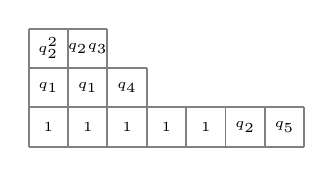
\begin{tikzpicture}[scale=.5] \coordinate (prev) at (0,0);
\foreach \dir in {7,3,2}{ \draw[help lines, line width = .25mm] (prev) -- +(0,1) coordinate (prev); \draw[help lines, line width = .25mm] (prev)+(0,-1) grid +(\dir,0); }; ;
\draw (.5,1.5) node {\tiny$q_1$};
\draw (.5,2.5) node {\tiny$q_2^2 $};
\draw (1.5,1.5) node {\tiny$q_1 $};
\draw (1.5,2.5) node {\tiny$q_2 q_3 $};
\draw (2.5,1.5) node {\tiny$q_4 $};
\draw (5.5,.5) node {\tiny$q_2 $};
\draw (6.5,.5) node {\tiny$q_5 $};
\draw (.5,.5) node {\tiny$1$};
\draw (1.5,.5) node {\tiny$1$};
\draw (2.5,.5) node {\tiny$1$};
\draw (3.5,.5) node {\tiny$1$};
\draw (4.5,.5) node {\tiny$1$};
\end{tikzpicture}~~\leftrightarrow
~~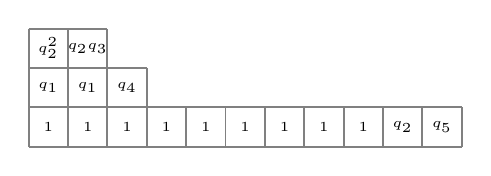
\begin{tikzpicture}[scale=.5] \coordinate (prev) at (0,0);
\foreach \dir in {11,3,2}{ \draw[help lines, line width = .25mm] (prev) -- +(0,1) coordinate (prev); \draw[help lines, line width = .25mm] (prev)+(0,-1) grid +(\dir,0); }; ;
\draw (.5,1.5) node {\tiny$q_1$};
\draw (.5,2.5) node {\tiny$q_2^2 $};
\draw (1.5,1.5) node {\tiny$q_1 $};
\draw (1.5,2.5) node {\tiny$q_2 q_3 $};
\draw (2.5,1.5) node {\tiny$q_4 $};
\draw (9.5,.5) node {\tiny$q_2 $};
\draw (10.5,.5) node {\tiny$q_5 $};
\draw (.5,.5) node {\tiny$1$};
\draw (1.5,.5) node {\tiny$1$};
\draw (2.5,.5) node {\tiny$1$};
\draw (3.5,.5) node {\tiny$1$};
\draw (4.5,.5) node {\tiny$1$};
\draw (5.5,.5) node {\tiny$1$};
\draw (6.5,.5) node {\tiny$1$};
\draw (7.5,.5) node {\tiny$1$};
\draw (8.5,.5) node {\tiny$1$};
\end{tikzpicture}
\]

\end{proof}

Viewing ${}_{n}F^{\lambda}$ as an $S_{n}$ module, one has
\[
{}_{n}F^{\lambda}\cong\bigoplus_{\mu\vdash n}\mathrm{Hom}_{S_{n}}(V^{\mu}%
,{}_{n}F^{\lambda})\otimes V^{\mu}.
\]
We will use the notation
\[
g_{\mu}^{\lambda}= \dim\mathrm{Hom}_{S_{n}}(V^{\mu},{}_{n}F^{\lambda}).
\]


%%% For any partition $\nu$, we will write $\nu\rightarrow\rho$ if one can attain
%%$\rho$ from $\nu$ by adding one cell. Then
%%\[
%%\mathrm{Res}_{S_{n-1}}^{S_{n}}V^{\rho}\cong\bigoplus_{\nu\rightarrow\rho
%%}V^{\nu}~~~\text{ and }~~~\mathrm{Ind}_{S_{n-1}}^{S_{n}}V^{\nu}\cong%
%%\bigoplus_{\nu\rightarrow\rho}V^{\rho}.
%%\]


\begin{lemma}
Let $\mu\vdash n$ and $\eta\vdash l < n$. Then for any $r \geq0$, we have
\begin{align*}
\dim\mathrm{Hom}_{S_{n}}( \mathrm{Ind}^{S_{n}}_{S_{l} \times S_{n-l}}  & (
V^{\eta} \otimes1_{n-l}) ,V^{\mu})\\
&  \leq\dim\mathrm{Hom}_{S_{n}} ( \mathrm{Ind}^{S_{n+r}}_{S_{l} \times
S_{n+r-l}} (V^{\eta} \otimes1_{n+r-l}), V^{\mu+r e_{1}}) .
\end{align*}

\end{lemma}

\begin{proof}
We will use the following Pieri rule: Let $1_{n}$ represent the trivial
representation for $S_{n}$. Then
\[
\mathrm{Ind}_{S_{l} \times S_{n-l}}^{S_{n} } (V^{\eta} \otimes1_{n-l})
\cong{\displaystyle\bigoplus_{%
\begin{array}
[c]{c}%
\mu_{1} \geq\eta_{1} \geq\mu_{2} \geq\cdots\geq\eta_{\ell(\mu)} \geq\mu
_{\ell(\mu)+1}\\
|\mu| = n
\end{array}
}} V^{\mu}.
\]
Note that if $V^{\mu}$ appears as an irreducible, the inequalities are then
also satisfied by
\[
\mu_{1} +r \geq\eta_{1} \geq\mu_{2} \geq\cdots\geq\eta_{\ell(\mu)} \geq
\mu_{\ell(\mu)+1}
\]
meaning $V^{\mu+r e_{1}}$ appears in $\mathrm{Ind}_{S_{l} \times S_{n+r-l}%
}^{S_{n} } (V^{\eta} \otimes1_{n+r-l})$.
\end{proof}

\begin{theorem}
For $\mu\vdash n$, $|\lambda| \leq n - \mu_{2}$ and $r \geq0$, we have
\[
g^{\lambda}_{\mu}= g^{\lambda}_{\mu+re_{1}}.
\]

\end{theorem}

\begin{proof}
We start with writing, as an $S_{n}$ module,
\[
{}_{n} F^{\lambda} = \bigoplus_{\text{ $\xi$ dominant}} \mathrm{Ind}%
_{S_{n,\mu}}^{S_{n}} {}_{n} (F^{\lambda})_{\xi}.
\]
Each subgroup can be written as $S_{n,\xi} = S_{\ell(\xi),\xi} \times
S_{n-\ell(\xi)}$, where now, by Proposition \ref{proptrivial}, $S_{n-\ell
(\xi)}$ acts trivially on ${}_{n} (F^{\lambda})_{\xi}$. We then have
\[
\mathrm{Ind}_{S_{n,\xi}}^{S_{n}} {}_{n} (F^{\lambda})_{\xi}= \mathrm{Ind}%
_{S_{\ell(\xi)} \times S_{n-\ell(\xi)} }^{S_{n}} ( \mathrm{Ind}_{S_{\ell
(\xi),\xi} }^{S_{\ell(\xi)}} {}_{n} (F^{\lambda})_{\xi}\otimes1_{n-\ell(\xi
)}),
\]
and from Lemma \ref{lemma2},
\[
\mathrm{Ind}_{S_{n+r,\xi}}^{S_{n}} {}_{n+r} (F^{\lambda})_{\xi}=
\mathrm{Ind}_{S_{\ell(\xi)} \times S_{n+r-\ell(\xi)} }^{S_{n}}( \mathrm{Ind}%
_{S_{\ell(\xi),\xi} }^{S_{\ell(\xi)}} {}_{n} (F^{\lambda})_{\xi}%
\otimes1_{n+r-\ell(\xi)}).
\]
It follows from the previous lemma that
\[
\dim\mathrm{Hom}_{S_{n}} ( \mathrm{Ind}_{S_{n,\xi}}^{S_{n}} {}_{n}
(F^{\lambda})_{\xi}, V^{\mu}) \leq\dim\mathrm{Hom}_{S_{n}}( \mathrm{Ind}%
_{S_{n+r,\xi}}^{S_{n}} {}_{n+r} (F^{\lambda})_{\xi}, V^{\mu+r e_{1}} ) ,
\]
and therefore
\[
g^{\lambda}_{\mu} \leq g^{\lambda}_{\mu+re_{1}}.
\]
From Theorem \ref{multigradedthm}, for $|\lambda| = m \leq n - \mu_{2}$ we
must have the equality
\[
\sum_{%
\begin{array}
[c]{c}%
\lambda\dashv n\\
\ell(\lambda)\leq k
\end{array}
}\dim{}_{k}F^{\lambda}\otimes\left(  g_{\mu}^{\lambda}-g_{\mu+re_{1}}%
^{\lambda}\right)  =0.
\]
This implies, as in Theorem \ref{Weyl-stability}, that $g_{\mu}^{\lambda} =
g_{\mu+re_{1}}^{\lambda}$.
\end{proof}

\section{Some conjectures related to stability}

In this section we will describe two conjectures that sharpen the results in
the previous sections. The first we call the quasi-freeness conjecture.

Let $\mathcal{R}_{k,n}$ and $p_{\alpha}$ be as in section 2. Let $d(\alpha)$
denote the degree of $p_{\alpha}$. Let $\mathcal{H}_{k,n}$ be the graded space
of $S_{n}$ harmonics which form an orthogonal complement to the ideal,
$\mathcal{I}_{k,n}$, generated by the $p_{\alpha}$ with $d(\alpha)>0.$

\begin{conjecture}
If $m\leq n$ and for each $\alpha$ with $d(\alpha)\leq m$ we have homogeneous
$h_{\alpha}\in\mathcal{H}_{k,n}$ such that $d(\alpha)+\deg(h_{\alpha})=m$, and
if
\[
\sum_{d(\alpha)\leq m}h_{\alpha}p_{\alpha}=0,
\]
then $h_{\alpha}=0$ for all $\alpha$ with $d(\alpha)\leq m$.
\end{conjecture}

We call the condition in the statement of the Lemma \textquotedblleft
quasi-freeness\textquotedblright. We will make a few observations which imply
the conjecture for all $k,n$ and $m\leq3$.

Write the sum that is $0$ out as%
\[
h_{0}+\sum_{d(\alpha)=1}h_{\alpha}p_{\alpha}+\cdots+\sum_{d(\alpha)=m-1}%
h_{\alpha}p_{\alpha}+\sum_{d(\alpha)=m}h_{\alpha}p_{\alpha}.
\]
Then by definition of $\mathcal{H}_{k,n}$, $h_{0}=0.$ Observing that the only
$S_{n}$--invariants in $\mathcal{H}_{k,n}$ are the constants and since
$h_{\alpha}$ is constant if $d(\alpha)=m$, we see that $\sum_{d(\alpha
)=m}h_{\alpha}p_{\alpha}$ is an $S_{n}$--invariant. If $m=1$ then we have
\[
\sum_{d(\alpha)=1}h_{\alpha}p_{\alpha}=0
\]
and if $m>1$ then
\[
-\sum_{d(\alpha)=m}h_{\alpha}p_{\alpha}=\sum_{d(\alpha)=1}h_{\alpha}%
p_{\alpha}+\cdots+\sum_{d(\alpha)=m-1}h_{\alpha}p_{\alpha}.
\]
Noting that if $d(\alpha)<m$ then $\deg h_{\alpha}\geq1$, one sees that the
projection onto the invariants of the right hand side of the equation is $0$.
Since the degrees of the $h_{\alpha}$ on the left hand side are $0$, the left
hand side is invariant. This implies that both sides of the equality are $0$
and, hence, in both cases $\sum_{d(\alpha)=m}h_{\alpha}p_{\alpha}=0$. Since
$m\leq n$, the $p_{\alpha}$ are linearly independent so $h_{\alpha}=0$ for
$d(\alpha)=m$. Notice that our observations now proves the conjecture for
$m=1$, so assume that $m\geq2$ and set
\[
L_{i}=\sum_{j=1}^{n}\frac{\partial}{\partial{}_{i}x_{j}}.
\]
Then, since $L_{i}h=0$ for $h\in\mathcal{H}_{k,n}$ and $L_{i}$ is a
derivation, we have for each $i$%
\[
-\sum_{d(\alpha)=1}h_{\alpha}L_{i}p_{\alpha}=\sum_{d(\alpha)=2}h_{\alpha
}L_{i}p_{\alpha}+\cdots+\sum_{d(\alpha)=m-1}h_{\alpha}L_{i}p_{\alpha}.
\]
The left hand side of the equation is $-nh_{\alpha_{i}}$ with $p_{\alpha_{i}%
}=\sum_{j=1}^{n}{}_{i}x_{j}$ and the right hand side is in the ideal, thus
$h_{\alpha}=0$ for $d(\alpha)=1$. This proves the conjecture for $m=2$. For
$m=3$ we are left with%
\[
\sum_{d(\alpha)=2}h_{\alpha}p_{\alpha}=0.
\]
In this case using the fact that a basis of the space of elements of degree
$1$ in $\mathcal{H}_{k,n}$ is given by
\[
\left\{  {}_{i}x_{j}-{}_{i}x_{j+1}|i=1,\dots,k, j=1,\dots,n-1\right\}
\]
one can prove that this implies that the vanishing of the sum implies that
$h_{\alpha}=0$ for all the pertinent $\alpha$. The argument is complicated and
will not generalize so we omit it.

If $\phi(q)$ is a polynomial in $q$ equal to $\sum\phi_{i}q^{i}$, then we set
$\phi(q)_{\leq m}=\sum_{i\leq m}a_{i}q^{i}$. The conjecture has the following corollary:

If $h_{k,n}(q)$ is the Hilbert series of $\mathcal{H}_{k,n}$ then%
\[
h_{k,n}(q)_{\leq n}=\left(  \prod_{r=1}^{n}\frac{(1-q^{r})^{\binom{r+k-1}%
{k-1}}}{(1-q)^{k}}\right)  _{\leq n}.
\]
In fact the conjecture implies a more precise formula. Setting $\mathcal{H}%
_{k,n}^{r}$ and $\mathcal{R}_{k,l}^{r}$ equal to the subspace of elements of
$\mathcal{H}_{k,n}$(resp. $\mathcal{R}_{k,l}^{r}$) homogenous of degree $r$
and for $\lambda\dashv n$,
\[
\mu_{\lambda,k,n}(r)=\dim\mathrm{Hom}_{S_{n}}(V^{\lambda},\mathcal{H}%
_{k,n}^{r}).
\]
and
\[
\tau_{_{\lambda,k,n}}(r)=\dim\mathrm{Hom}_{S_{n}}(V^{\lambda},\mathcal{R}%
_{k,n}^{r}).
\]
Then%
\[
\sum_{r=0}^{m}\mu_{\lambda,k,n}(r)q^{r}=\left(  \prod_{r=1}^{m}(1-q^{r}%
)^{\binom{r+k-1}{k-1}}\sum_{r=1}^{m}\tau_{_{\lambda,k,n}}(r)q^{r}\right)
_{\leq m}.
\]
for all $m\leq n$. The arguments above show that this formula is proved for
$m\leq3$. We note that it is not even obvious that the right side of these
equations has positive coefficients. In the case of $k=2$ this conjecture
gives a simple interpretation of the Frobenius characteristic of the diagonal
Harmonics of Garsia and Haiman to degree $n$ \cite{qLagrange}. This conjecture
has been checked for $k=2,$ $n\leq6$ and for $n=7,m\leq4$.

The second conjecture involves lead monomials of Gr\"{o}bner bases. Order the
variables as
\[
x_{1}\leq y_{1}\leq\cdots\leq x_{n}\leq y_{n}.
\]
Let $G_{k,n}$ be the Gr\"{o}bner basis for $\mathcal{I}_{k,n}$. Let $LG_{k,n}$
be the set of leading monomials of $G_{k,n}$ and let $LG_{k,n}^{\leq m}$ be
the set of leading monomials of total degree at most $m$.

\begin{conjecture}
$LG_{k,n}^{\leq m}=LG_{k,m}^{\leq m}.$
\end{conjecture}

This conjecture has also been checked for $k=2$ $,n\leq6$ and for $k=2,$ $n=7$
and $m \leq4$.

Using the theory of Gr\"{o}bner Bases one sees that this conjecture implies:
If $h_{k,n}$ is the Hilbert series of the coinvariants of degree $k$ for the
$k$-fold diagonal action of $S_{n}$ and if $m < n$, then
\[
\left(  h_{k,n}\right)  _{\leq m}=\left(  \frac{h_{k,m}}{(1-q)^{k(n-m)}%
}\right)  _{\leq m}.
\]


\bibliographystyle{amsplain}
\bibliography{stabilizations}

{\small  \noindent\newline Marino Romero\newline University of California, San
Diego\newline Department of Mathematics \newline\emph{E\--mail}: \texttt{mar007@ucsd.edu} 
}
\newline{\small  \noindent\newline Nolan
Wallach\newline University of California, San Diego\newline Department of
Mathematics  \newline\emph{E\--mail}: \texttt{nwallach@ucsd.edu} 
}


\end{document}